\section{Specifikationer} \label{ch4_specs}
FIR-filteret vælges til at være af type 1, altså er filterordenen $M$ lige og impulsresponsen $h[n]$ er symmetrisk, så $h[n] = h[M - n]$. Filteret har 2 knækfrekvenser $\omega_{c_1}$ og $\omega_{c_2}$ i rad/s, som vælges til at ligge symmetrisk omkring $\omega_2$, der skal elimineres ved hjælp af filteret:
\begin{align*}
\omega_{c_1} &= \omega_2 - \delta, \\
\omega_{c_2} &= \omega_2 + \delta,
\end{align*}

hvor $\delta$ vælges til at være $\frac{\pi}{15}$. Filteret designes dermed som et båndstopfilter med ovenstående knækfrekvenser. Den ideelle amplituderespons $|H_d(\text{e}^{j\omega})|$ er skitseret på figur \ref{fig:ideel_amp_respons} ud fra de opstillede specifikationer.
\begin{figure}[H]
    \centering
    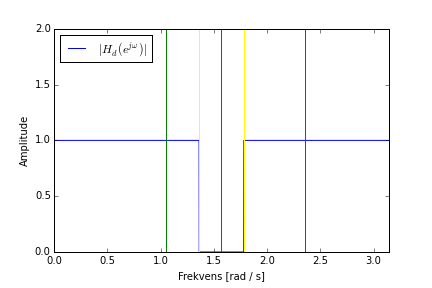
\includegraphics[width = 0.6\textwidth]{figures/Filter/ideel_amp_respons.PNG}
    \caption{Den ideelle amplituderespons for filteret. De to grønne streger markerer $\omega_1$ og $\omega_3$, som skal beholdes, og de to gule streger markerer $\omega_{c_1}$ og $\omega_{c_2}$, som ligger symmetrisk omkring den røde streg, der markerer $\omega_2$, som skal elimineres.}
    \label{fig:ideel_amp_respons}
\end{figure}
